% \iffalse
\let\negmedspace\undefined
\let\negthickspace\undefined
\documentclass[journal,12pt,twocolumn]{IEEEtran}
\usepackage{cite}
\usepackage{amsmath,amssymb,amsfonts,amsthm}
\usepackage{algorithmic}
\usepackage{graphicx}
\usepackage{textcomp}
\usepackage{xcolor}
\usepackage{txfonts}
\usepackage{listings}
\usepackage{enumitem}
\usepackage{mathtools}
\usepackage{gensymb}
\usepackage{comment}
\usepackage[breaklinks=true]{hyperref}
\usepackage{tkz-euclide} 
\usepackage{listings}
\usepackage{gvv}                                        
\def\inputGnumericTable{}                                 
\usepackage[latin1]{inputenc}                                
\usepackage{color}                                            
\usepackage{array}                                            
\usepackage{longtable}                                       
\usepackage{calc}                                             
\usepackage{multirow}                                         
\usepackage{hhline}                                           
\usepackage{ifthen}                                           
\usepackage{lscape}
\newtheorem{theorem}{Theorem}[section]
\newtheorem{problem}{Problem}
\newtheorem{proposition}{Proposition}[section]
\newtheorem{lemma}{Lemma}[section]
\newtheorem{corollary}[theorem]{Corollary}
\newtheorem{example}{Example}[section]
\newtheorem{definition}[problem]{Definition}
\newcommand{\BEQA}{\begin{eqnarray}}
\newcommand{\EEQA}{\end{eqnarray}}
\newcommand{\define}{\stackrel{\triangle}{=}}
\theoremstyle{remark}
\newtheorem{rem}{Remark}
\begin{document}

\bibliographystyle{IEEEtran}
\vspace{3cm}

\title{11.9.4.7}
\author{EE23BTECH11063 - Vemula Siddhartha
}
\maketitle
\newpage
\bigskip

\renewcommand{\thefigure}{\theenumi}
\renewcommand{\thetable}{\theenumi}
\textbf{Question}:\\
Find the sum to $n$ terms of the series:\\
    $1^2+\brak{1^2+2^2}+\brak{1^2+2^2+3^2}+...$
    \\
\textbf{Solution:}
%\fi
\begin{table}[h!]    
    \centering
    \begin{tabular}[12pt]{ |c| c|}
    \hline
    \textbf{Symbol} & \textbf{Description}\\ 
    \hline
    $ f\brak{x} $ & Function \\
    \hline 
    $ G\brak{f} $ & Fourier Transform of the function $ f\brak{x} $ \\
    \hline
    $ f^*\brak{x} $ & Complex Conjugate of $ f\brak{x} $ \\
    \hline
    $ G^*\brak{f} $ & Complex Conjugate of $ G\brak{f} $ \\
    \hline
    Im$ \brak{ G \brak{ f } }$ & Imaginary Part of $ G\brak{f} $ \\
    \hline
    \end{tabular}
    \caption{Variables Used}
    \label{tab10.5.3.9.1}
  \end{table}
\begin{align}
    y\brak{n}&=1^2+\brak{1^2+2^2}+\brak{1^2+2^2+3^2}+...
\end{align}
Let,
\begin{align}
    x\brak{n}&=\brak{n+1}^2u\brak{n}\\
    \implies y\brak{n}&=x\brak{n}*u\brak{n}*u\brak{n}\\
    Y\brak{z}&=X\brak{z}\brak{U\brak{z}}^2
\end{align}
From \eqref{eq:11.9.5.26.3},
\begin{align}
    n^2u\brak{n}\system{Z}\frac{z^{-1}\brak{1+z^{-1}}}{\brak{1-z^{-1}}^3}\;\;\cbrak{\abs{z}>1}
\end{align}
Using \eqref{eq:shiftk},
\begin{align}
    \brak{n+1}^2u\brak{n}&\system{Z}\frac{1+z^{-1}}{\brak{1-z^{-1}}^3}\;\;\cbrak{\abs{z}>1}\label{eq:11.9.4.7.1}
\end{align}
From \eqref{eq:11.9.4.7.1},
\begin{align}
    Y\brak{z}&=\brak{\frac{1+z^{-1}}{\brak{1-z^{-1}}^3}}\brak{\frac{1}{1-z^{-1}}}^2\\
    &=\frac{1+z^{-1}}{\brak{1-z^{-1}}^5}\\
    &=\frac{1}{\brak{1-z^{-1}}^5}+\frac{z^{-1}}{\brak{1-z^{-1}}^5}\;\cbrak{\abs{z}>1}
\end{align}
From \eqref{eq:11.9.5.26.12}, using \eqref{eq:shiftk},
\begin{align}
    \frac{\brak{n+1}\brak{n+2}\brak{n+3}\brak{n+4}}{24}u\brak{n}&\system{Z}\frac{1}{\brak{1-z^{-1}}^5}\label{eq:11.9.4.7.2}\cbrak{\abs{z}>1}\\
    \frac{\brak{n}\brak{n+1}\brak{n+2}\brak{n+3}}{24}u\brak{n}&\system{Z}\frac{z^{-1}}{\brak{1-z^{-1}}^5}\label{eq:11.9.4.7.3}\cbrak{\abs{z}>1}
\end{align}
From \eqref{eq:11.9.4.7.2} and \eqref{eq:11.9.4.7.3}, taking the Inverse Z Transform,
\begin{align}
    y\brak{n}&=\brak{\frac{\brak{n+1}\brak{n+2}\brak{n+3}\brak{n+4}}{24}u\brak{n}}\notag\\
    &\;+\brak{\frac{\brak{n}\brak{n+1}\brak{n+2}\brak{n+3}}{24}u\brak{n}}\\
    \implies y\brak{n}&=\frac{\brak{n+1}\brak{n+2}^2\brak{n+3}}{12}u\brak{n}
\end{align}
\begin{figure}[h!]
    \centering
    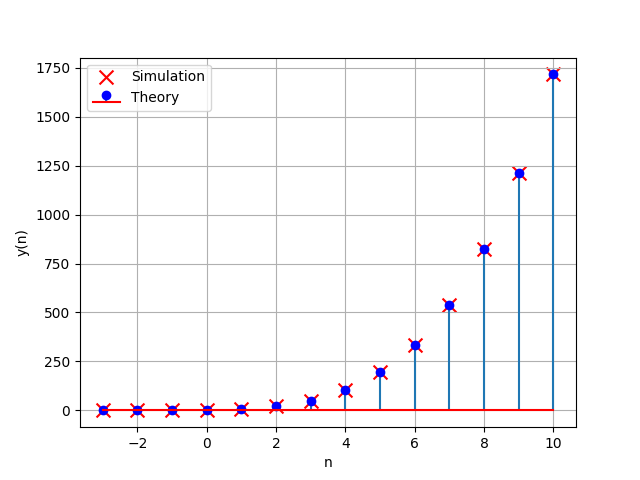
\includegraphics[width=\linewidth]{figs/Figure_1.png}
    \caption{Stem Plot of $y\brak{n}$}
\end{figure}
\end{document}